\chapter{Systembestandteile}
\label{chap:funkt}
Um die Installation mit ihren einzelnen Komponenten besser verstehen zu können, wird an dieser Stelle kurz auf die für ERPNext entwickelten Bestandteile eingegangen.

\section{Frappé Framework}
Frappé, die Firma hinter ERPNext hat eigens für das System ein eigenes Web-Framework entwickelt (\vgl \cite{FrappeIo}). Dieses in Python und JavaScript geschriebene Tool bildet die Grundlage für die Architektur von ERPNext. Es vereint sowohl Backend- als auch Frontend-Komponenten und liefert somit viele nützliche Funktionen, um nicht komplett \glqq from scratch\grqq\ starten zu müssen. Dazu zählt unter anderem eine REST-Schnittstelle, ein Admin-\gls{ui}, eine Benutzersteuerung, Unterstützung für E-Mail-Accounts sowie eine modulare Architektur.

\section{Frappé Bench}
Die Frappé Bench ist ein \gls{cli} um verschiedene Seiten und Apps zu verwalten (\vgl \cite{GhBench}). 
Eine App bezeichnet in diesem Kontext eine im Frappé Framework programmierte Anwendung, wie beispielsweise ERPNext. Diese kann dann auf einer Seite (= Webseite) installiert werden, die von der Bench verwaltet wird. So können auch mehrere Instanzen einer App auf verschiedenen Seiten deployed werden, was bei einem \gls{erp}-System sinnvoll ist. Durch die Verwaltungsfunktionen der Bench können ähnlich den Paketverwaltungstools von Linux-Betriebssystemen Apps jederzeit einheitlich installiert, deinstalliert und geupdatet werden.\\
Da die Bench als \gls{cli}-Anwendung kein \gls{gui} besitzt, wurde extra dafür eine Software namens Bench Manager geschrieben (\vgl \cite{GhBenchManager}). Diese basiert ebenso auf dem Frappé Framework und lässt in begrenztem Umfang die gleichen Funktionen wie das Kommandozeilen-Programm erledigen. \\
Darüber hinaus bietet diese Softwarekomponente komfortable Dienste, wie beispielsweise die Einrichtung eines SSL-Zertifikats für Seiten mit Let's Encrypt an (\vgl \cite{GhBenchSsl}).
\begin{figure}
  \centering
  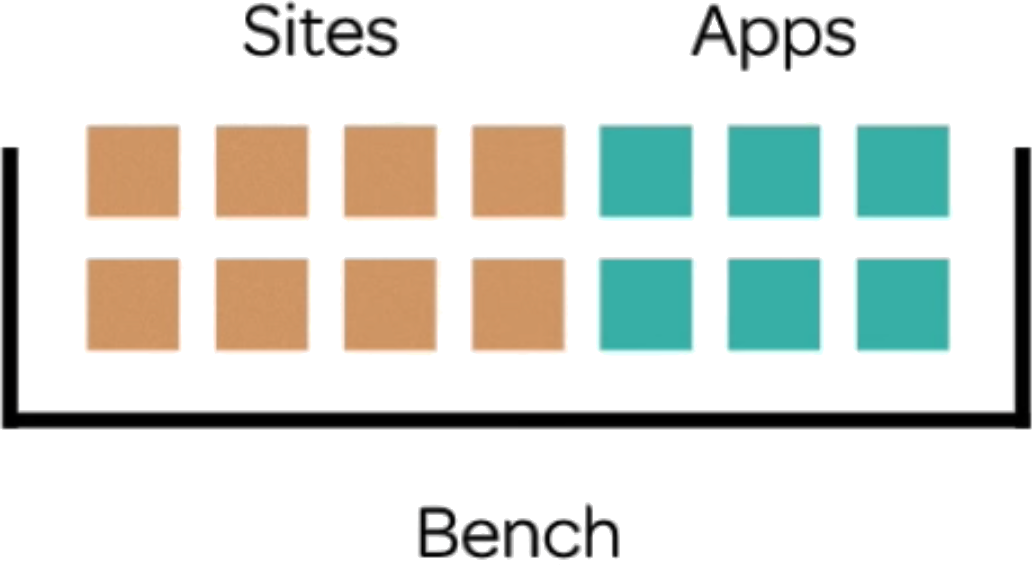
\includegraphics[width=0.5\textwidth]{Bilder/Bench_vereinfacht.png}
  \caption{Bench (vereinfacht)}
  \label{fig:benchVereinfacht}
\end{figure}
\begin{figure}
  \centering
  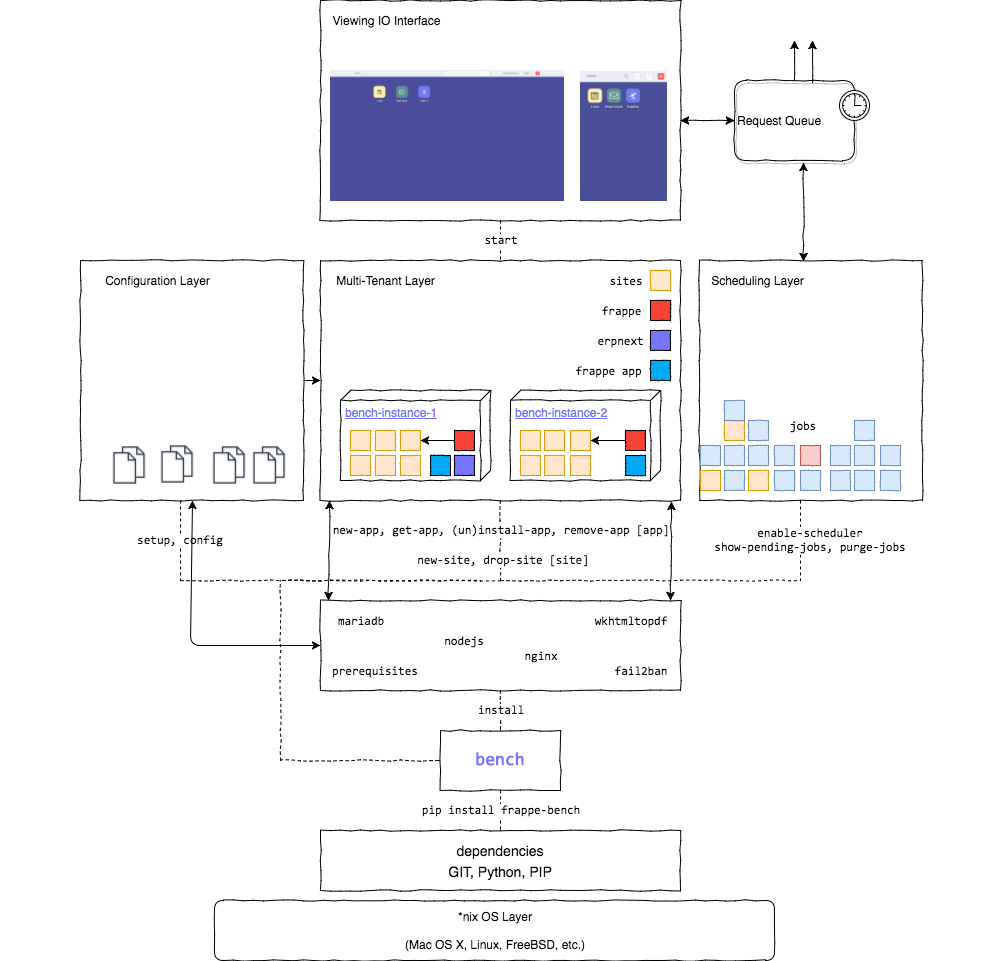
\includegraphics[width=\textwidth]{Bilder/Bench.png}
  \caption{Architektur der Bench}
  \label{fig:bench}
\end{figure}